\documentclass[9pt]{beamer-control}
\usepackage{beamer-control-prac}
\begin{document}
\TOPIC[2]{Feedback Control}
\CONCEPT[4]{Week 4: Feedback design}

\begin{frame}
\frametitle{Introduction}
In this practical, the process of characterising a plants output response will be used to derive initial gains for a PID controller for both the angular displacement and velocity of the inertia disk.

\vfill

This practical will consist of the following parts:
\begin{itemize}
\item Controlling angular displacement
\item Controlling angular velocity
\end{itemize}
\end{frame}



\SUBCONCEPT{Controlling angular displacement}

\begin{frame}{Tuning a displacement controller}
In previous weeks we have characterised the angular output of the QUBE inertia disk as an Integrator with Time Delay (ITD) model. From this output characterisation we can use offline tuning laws to set $K_p$, $K_i$, and $K_d$ which can be found at the end of this document.

\begin{enumerate}
\item Find the ITD parameters $a$ and $L$ of the inertia disk model 
\item Using the Ziegler-Nichols tuning law, calculate the corresponding PID gains
\item Run the plant and controller with these gains and assess the performance to a step input of $\tfrac{\pi}{2}$
\item Repeat with the ITD Chien-Hrones-Reswick tuning law and compare
\end{enumerate}

Which offers the better performance?


\end{frame}




\SUBCONCEPT{Controlling angular velocity}

\begin{frame}{Tuning a speed controller}
Suppose we instead wish to control the angular velocity of the inertia disk to introduce `speed control'. 

\begin{enumerate}
	\item First we need to measure the velocity of the inertia disk, which can be facilitated through adding in a low-pass filter and a Derivative block, additionally connect this to a Scope
	\item You will see after running the Simulink file that In this case the ITD model is not a great fit, we instead need to use the First Order Time Delay (FOTD) model which is on the following slide
	\item Calculate the FOTD parameters $a$, $T$, and $L$, and using the FOTD Chien-Hrones-Reswick tuning law calculate the corresponding PID gains
	\item Run the plant and controller with these gains and assess the performance to a step input of $1$
	\item Repeat with the Cohen-Coon tuning law and compare
	
\end{enumerate}

\textcolor{red}{Simulink diagram}

\end{frame}

\begin{frame}{Tuning a speed controller}
	\begin{figure}
	\centering
	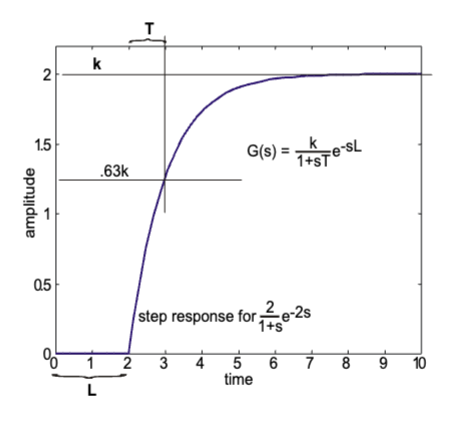
\includegraphics[width=8cm]{prac4_fotd.png}
	\caption{First Order Time Delay (ITD) model.}
\end{figure}
\end{frame}


\SUBCONCEPT{Tuning laws}

\begin{frame}{Tuning laws}
	\centering
	The time constants relate to the gains by $K_i= \frac{K_p}{T_i}$ and $K_d = K_p T_d$\\
	\vfill
	
	\begin{columns}
		\begin{column}{0.5\textwidth}
			ITD tuning laws
			\begin{table}
				\centering
				\begin{tabular}{|c|c|c|}
					\hline
					$K_p$ & $T_i$ & $T_d$\\
					\hline
					$\frac{1.2}{a}$ & $2L$ & $\frac{L}{2}$\\
					\hline	
				\end{tabular}
				\caption{Ziegler-Nichols tuning law}
			\end{table}
			
			\begin{table}
				\centering
				\begin{tabular}{|c|c|c|}
					\hline
					$K_p$ & $T_i$ & $T_d$\\
					\hline
					$\frac{0.95}{a}$ & $2.4 L$ & $0.42 L$\\
					\hline	
				\end{tabular}
				\caption{ITD Chien-Hrones-Reswick tuning law (0\% overshoot)}
			\end{table}
		\end{column}
		\begin{column}{0.5\textwidth} 
			
			FOTD tuning laws
			\begin{table}
				\centering
				\begin{tabular}{|c|c|c|}
					\hline
					$K_p$ & $T_i$ & $T_d$\\
					\hline
					$\frac{0.6}{a}$ & $T$ & $\frac{L}{2}$\\
					\hline	
				\end{tabular}
				\caption{FOTD Chien-Hrones-Reswick tuning law (0\% overshoot)}
			\end{table}
			
			\begin{table}
				\centering
				\begin{tabular}{|c|c|c|}
					\hline
					$K_p$ & $T_i$ & $T_d$\\
					\hline
					\tiny{$\frac{1.35}{a}\left(1 + \frac{0.18 \tau}{1-\tau} \right)$} & \tiny{$ L\left( \frac{2.5-2\tau}{1-0.39\tau} \right) $} & \tiny{$L \left( \frac{0.37-0.37\tau}{1-0.81\tau} \right)$}\\
					\hline	
				\end{tabular}
				\caption{Cohen-Coon tuning law where $\tau=\frac{L}{L+T}$}
			\end{table}
		\end{column}
	\end{columns}
	
	
\end{frame}


\begin{frame}{Next week}
	This week you characterised the angular displacement and velocity of the inertia disk system as ITD and FOTD models respectively to derive appropriate PID gains using tunings laws.
	
	Next week we will begin the practical module on the frequency domain, move onto the compound pendulum QUBE system, and look at further control methods.
\end{frame}



\end{document}
